\section{Brillanza superficiale}\label{sec:brillanza-superficiale}
Un altro parametro importante della galassie è la loro brillanza superficiale (surface brightness, SB): questa altro non è che la distribuzione bidimensionale della materia luminosa sul piano del cielo, quindi la magnitudine per unità di area. Come facciamo a calcolare i profili di brillanza superficiale? Per farlo si costruiscono le isofote (ossia anelli di profilo caratterizzata dalla stessa brillantezza), si calcola la brillanza in ogni anello e infine si plottano i profili di brillanza superficiale (magnitudine - raggio), rappresentati in figura~\ref{fig:profili-brillanza}.

\begin{figure}
    \centering
    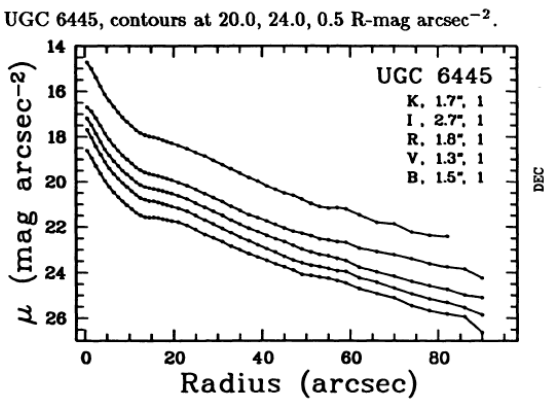
\includegraphics[width = 0.5 \textwidth]{immagini/profili-di-brillanza.png}
    \caption{Profili di brillanza, costruiti plottando la magnitudine a raggi diversi (quindi studiando la magnitudine delle isofite).}
    \label{fig:profili-brillanza}
\end{figure}

Si è osservato che quasi tutti i profili di brillanza delle galassie (sia ellittiche sia a spirale) seguono il profilo di Sersic, descritto dalla seguente equazione:

\begin{equation*}
    I(r) = I_0 \; e^{-b_n \big(\frac{r}{r_e}\big)^\frac{1}{n}}
\end{equation*}

in cui $I(r)$ è la brillantezza superficiale, $I_0$ è la brillantezza centrale, $r_e$ è il raggio effettivo (ossia il raggio contenente il 50\% della luce proiettata), $b_n$ una costante e $n$ è l'indice di concentrazione (compreso fra $1$ e $10$).

Le galassie ellittiche sono caratterizzate da un cosiddetto "profilo Vaucoulerurs", corrispondente a n=4, mentre le galassie a spirale hanno un profilo di tipo esponenziale, corrispondente a n=1. 